 
To evaluate interactive smart shelf, we tested it more than one time in real world scenarios. We found some strengths and weakness after the evaluation of our project. Moreover we did seven activities during evaluation that are listed the table below.

\subsection{Strength} 
\begin{description}
  \item[$\bullet$] The design of drawers are reliable, long lasting and system has a Multiple User Interface for multiple users.
   \item[$\bullet$] In service mode, color of LED's follows cultural analogy, i.e. Red (no item), Blue (have an item) and Yellow (<=half amount) in each drawer.
   \item[$\bullet$] If there isn't any item in drawers, system send notification email to operator.
   \item[$\bullet$] Web application smoothly start service mode that depicts the current state of smart shelf.
   \item[$\bullet$] More than one user can search items simultaneously.
   \item[$\bullet$] Using QR-Code user can get detail information of items i.e. capacity of resistors etc.
   \end{description}
\subsection{weakness}
\begin{itemize}
  \item LED's inside drawer is not clearly visible for visualization.
        \subsection{solution}
         Use huge diffused LED's (10mm diameter). These are really bright so these can be seen in daytime. These have 465-470nm wavelength, 3.0-3.4V forward voltage and require 20mA current. Typical brightness is 1000mcd instead of using 5mm.
  \item Load Cell is fix with plastic plate inside drawer. Sometimes Load Cell isn't measure correct weight owing to around space between plate and drawer.
  		 \subsection{solution}
  		 Inside drawer there should not any space between the edges of plate and drawer.
  \item  Power supply is also an issue, sometimes some LED's isn't blink or ON just because of insufficient power supply.
  	   \subsection{solution}
  	    We can power up Micro Controller using an AC to DC adapter plugged into the barrel connector.The barrel connector can be supplied 7-12V or can use battery greater than 5V. 
  \item Place a QR Code outside of each small drawer is also a problem.
  	   \subsection{solution}
  	    NFC \footnote{Abbr. Near Field Communication} Tags are one of the new tool that could be replace QR Code. NFC Tags are small in size so can easily be placed outside of each drawer. Most important NFC Tags are more secure, flexible, and easier to configure than QR Codes. It is also easy to make changes and edit existing NFC Tags rather than QR Codes. One last thing unlike QR Code, NFC Tags do not require an extra application. We can also use SnapTag.
 %
\begin{figure}
	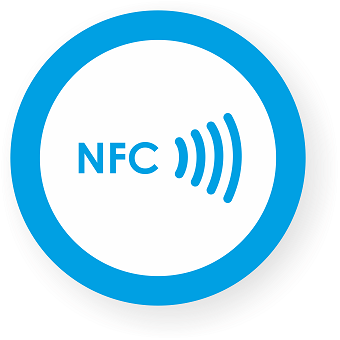
\includegraphics[width=0.9\columnwidth]{figures/NFCTag}
	\caption{NFC Tag}~\label{fig:NFC}
\end{figure}
%

\end{itemize}
\subsection{Best Scenarios} 
  The project works best when search any item in drawer and scan QR Code to get further detail via Web App. Moreover proper communication is establish between Web App and Micro Controller via MQTT protocol. 
\subsection{User Testing} 
We tried Web App Smart Shelf with different users and observed when they were doing these activities. These activities are listed in table.
%
\begin{figure}
	\includegraphics[width=1.1\columnwidth]{figures/Table}
	\caption{}~\label{fig:table}
\end{figure}
%
\\
We tested all these activities with different 4 participants and got feedback. We recorded all data of four different participants in this section. The participants were from different age groups range from 20 to 29 years old people some were employee and some were students at the University of Saarland. For each participant performed each activity 10 times as mention in table. Then we evaluated the number of successful observations, false results and no response. We would discuss the results corresponding to each activity and the percentage of successful observations when our system was perfectly fine and when a false detection happened and what might be the possible reasons of false results.

For activity 1 and 5, we found our system is working properly in almost 88 percent cases because participants were intentionally performing.
While for activity 2, the system was relatively less accurate as compared to the first activity. More than one time the system did not measured correct weight. In 70 percent cases the system measured the weight of items correctly but 21 percent the system failed to measure quantity of items. This activity was dependent upon weight measurement. Sometimes load sensor interpret wrong weight. For example with 3rd participant we achieved the success rate  81 percent as compared to the 2nd one. 
Meanwhile activity 6 had high percentage of successful cases with 99 percent among the other all activities.
While performing activity 3, the success ratio was 88 percent that was almost similar with activity 5, 86 percent success rate.
As we went further and test activity 4, achieved success ratio over 96 percent, 4 percent cases was failed because of incorrect operations performed by novice users.

In Contrast, the result of activity 7 was worst among all of above mentioned activities as 55 percent cases was failed because of inefficient power supply. Participants gave bad feedback when they stopped service mode the LED's were still blinking and system became unresponsive. Sometimes some LED's were ON when service mode was started. 
At the end we conclude overall success rate of our Interactive Smart Shelf Web App in the light of these 7 activities was 90 percent. We found more than 85 percent of cases our system was working perfectly fine as shown in fig (5). 
%
\begin{figure}
	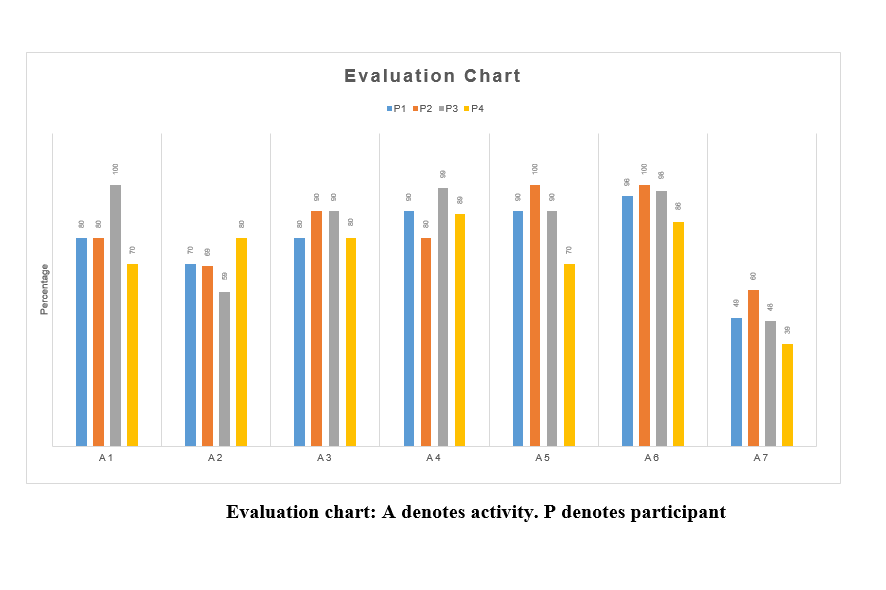
\includegraphics[width=1.1\columnwidth]{figures/Chart}
	\caption{}~\label{fig:Chart}
\end{figure}
%

This figure represent the overall evaluation report in form of bar chart. But 15 percent was unsatisfied result owing to some reasons that is mention above.
